\section{Resultados}

\subsection{Simpson dataset}

\subsubsection{Modelos con embedding personalizado}

Los modelos descritos previamente en la sección \ref{sec:deepModels} se implementan como clasificadores para identificar cuál de los personajes principales de Los Simpson dijo un diálogo específico. En este caso se identifican como personajes principales Bart, Homer, Lisa y Marge, siendo las clases 0, 1, 2, 3 respectivamente. Se almacenan los resultados y se muestran los siguientes resultados promediando según modelo, tamaño del embedding y longitud de la secuencia de entrada a la red.\\

\begin{figure}[H]
    \centering
    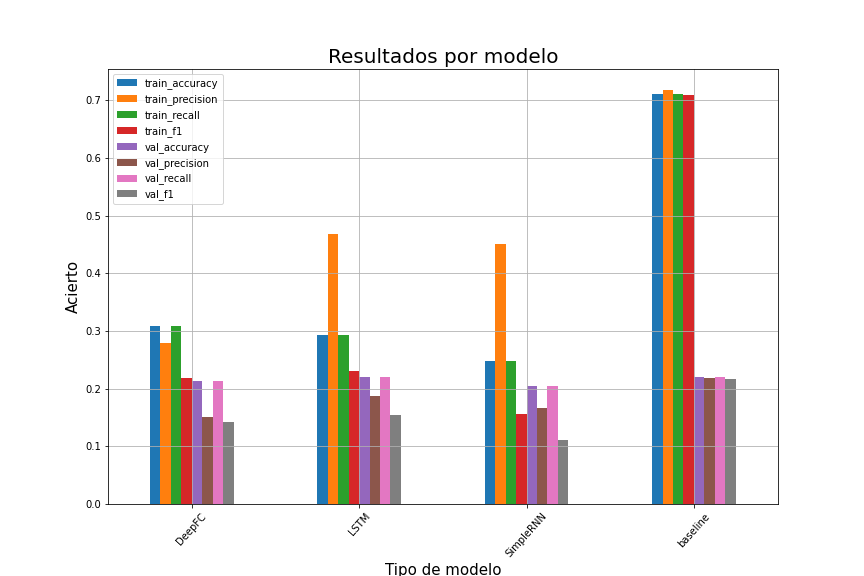
\includegraphics[width=0.9\textwidth]{results/friends/deepModels/sim_res_deep_model.png}
    \caption{Resultados por tipo de modelo}
    \label{fig:sim_deep_model}
\end{figure}

Según la figura \ref{fig:sim_deep_model}, es evidente que el modelo de tipo \textit{baseline} incurre rápidamente en \textit{overfitting}, pues su acierto en los datos de entrenamiento es muy bueno, pero en los de validación es pésimo. En cuanto a los otros modelos su rendimiento es relativamente parejo, destacando una muy buena precisión por parte de los modelos recurrentes  (LSTM y Simple RNN).\\

\begin{figure}[H]
    \centering
    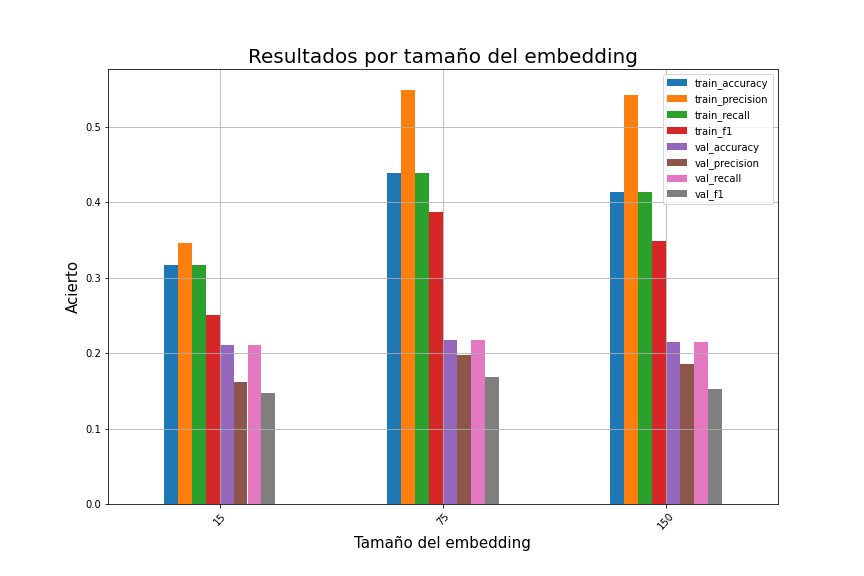
\includegraphics[width=0.9\textwidth]{results/friends/deepModels/sim_res_deep_em_size.png}
    \caption{Resultados por tamaño del embedding}
    \label{fig:sim_deep_em_size}
\end{figure}

Ahora bien, se desea comparar el efecto de los diferentes tamaños de embedding implementados, los cuales corresponden a 15, 75 y 150. Nuevamente, resulta evidente (\textit{véase fig. \ref{fig:sim_deep_em_size}}) que el embedding de tamaño 150 tiende a sobre ajustarse más a los datos de entrenamiento. No obstante, alcanza a dar un resultado ligeramente mejor que los de 15 y 75.\\

\begin{figure}[H]
    \centering
    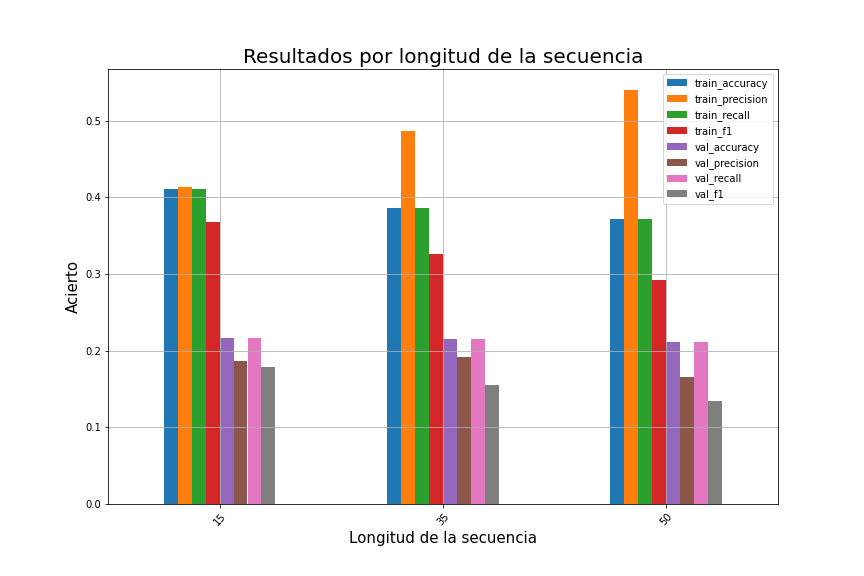
\includegraphics[width=0.9\textwidth]{results/friends/deepModels/sim_res_deep_seq_len.png}
    \caption{Resultados por el tamaño de la secuencia}
    \label{fig:sim_deep_seq_len}
\end{figure}

Finalmente, se desea comparar el efecto de utilizar secuencias de diferente tamaño (15, 35, 50). Los resultados en general son bastante similares favoreciendo un poco el f1 score de secuencias de tamaño 15.\\

Para análisis posteriores, se extrae el mejor modelo con base en el f1 score. Con este modelo se obtienen predicciones sobre datos de validación y de entrenamiento y se reentrena utilizando estos dos grupos de datos para predecir finalmente sobre los datos de test. Con base en todos estas predicciones se obtienen los siguientes resultados:

\begin{itemize}
    \item \textbf{Entrenamiento:}
    \input{results/simpson/deepModels/Train.txt}
    
    \begin{figure}[H]
        \centering
        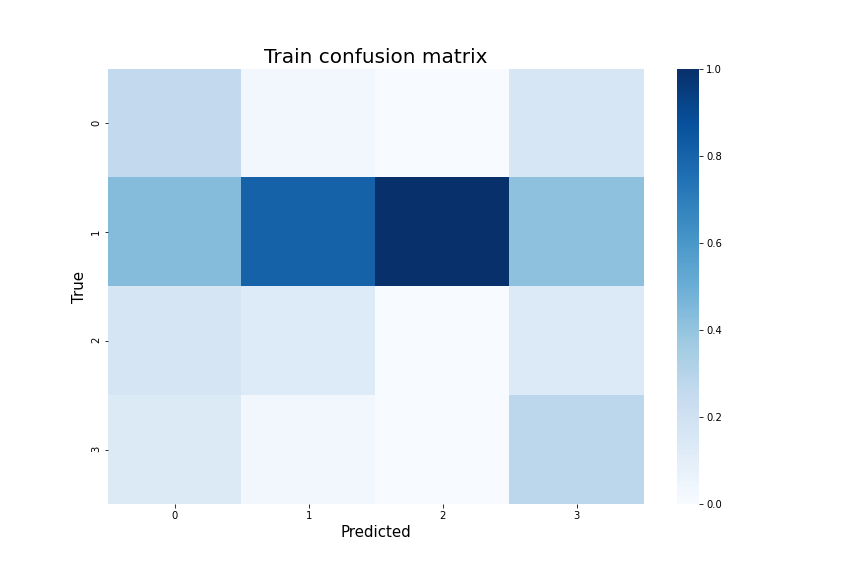
\includegraphics[width=0.9\textwidth]{results/simpson/deepModels/Train.png}
        \caption{Matriz de confusión para entrenamiento en Los Simpson}
        \label{fig:my_label}
    \end{figure}
    
    En el caso de la clase 1 correspondiente a Homer, se puede ver un recall muy bajo, lo que indica la baja certeza al clasificar un modelo como de su clase. Las métricas de las otras clases son ligeramente mejores, especialmente Bart y Marge, edn donde se aprecia un F1 score bastante bueno. En cuanto a la matriz de confusión, se puede ver que en algunos casos la diagonal está más cargada, no obstante, puede ser mejor.
    
    \item \textbf{Validación:}
    \input{results/simpson/deepModels/Validation.txt}
    
    \begin{figure}[H]
        \centering
        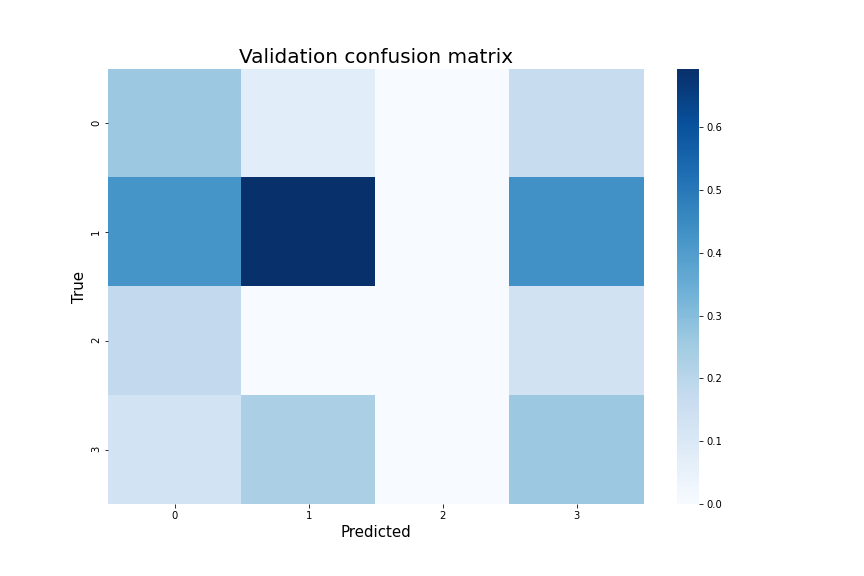
\includegraphics[width=0.9\textwidth]{results/simpson/deepModels/Validation.png}
        \caption{Matriz de confusión para validación en Los Simpson}
        \label{fig:my_label}
    \end{figure}
    
    Se puede apreciar un buen recall tanto para Bart como para Marge al igual que en entrenamiento. Los resultados en general son muy similares a los obtenidos en la etapa previa, como era de esperarse. 
    
    \item \textbf{Test:}
    \input{results/simpson/deepModels/Test.txt}
    
    \begin{figure}[H]
        \centering
        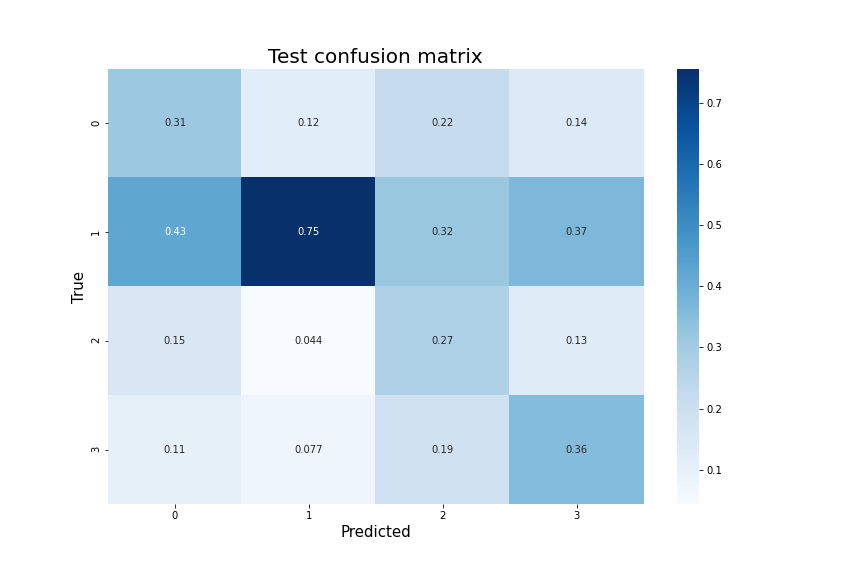
\includegraphics[width=0.9\textwidth]{results/simpson/deepModels/Test.png}
        \caption{Matriz de confusión para test en Los Simpson}
        \label{fig:my_label}
    \end{figure}
    
    En este caso se puede ver una importante y notable mejora en las clases que venían presentando problemas (Homer y Lisa). Se puede apreciar también una mejora en la distribución de la clasificación de la matriz de confusión aunque aún con puntos débiles especialmente en la clase 0 y 3, las cuales antes tenían mejores resultados
    
\end{itemize}

\subsubsection{Modelos con embedding dentro de la red}
La tabla \ref{tab:em_simpsons_global} presenta los resultados de los tipos de modelos considerados para el problema de clasificación del conjunto de datos de \textit{Los Simpsons}. Los resultados de la tabla \ref{tab:em_simpsons_global} provienen de la evaluación del conjunto de prueba sobre el mejor modelo de cada uno de los tipos que fueron puestos a prueba. En términos generales se puede decir que los modelos logran captar suficiente información como para realizar una clasificación dado que su \textit{accuracy} es mayor del 25\% esperado en un clasificador completamente aleatorio. Por otra parte, se tienen los valores de \textit{precision} y \textit{recall} que se combinan en la puntuación F1. Para la \textit{precision} se puede notar que supera el 60\% para todos los tipos de modelos, lo cual indica que estos tienden a presentar un menor número de falsos positivos. Sin embargo, el \textit{recall}, que en ningún caso supera el 40\%, indica que los modelos tienden a presentar falsos negativos.

\begin{table}[H]
    \centering
    \csvreader[%
    tabular={|c|c|c|c|c|},
    table head=\hline \textbf{Modelo} & \textbf{Accuracy} & \textbf{Precision} & \textbf{Recall} & \textbf{F1} \\ \hline,
    late after line=\\ \hline,
    respect underscore = true
    ]%
    {data/results/simpsons_models.csv}%
    {model=\model, accuracy=\acc, precision=\prec, recall=\rec, F1=\fone}
    {\model & \acc & \prec & \rec & \fone}
    \caption{Métricas de evaluación sobre datos de prueba de \textit{Los Simpsons} para los mejores modelos de cada tipo.}
    \label{tab:em_simpsons_global}
\end{table}


\begin{table}[H]
    \centering
    \csvreader[%
    tabular={|c|c|c|c|},
    table head=\hline \textbf{Clase} & \textbf{Precision} & \textbf{Recall} & \textbf{F1} \\ \hline,
    late after line=\\ \hline,
    respect underscore = true
    ]%
    {data/results/simpsons_train.csv}%
    {class=\class, precision=\prec, recall=\rec, F1=\fone}
    {\class & \prec & \rec & \fone}
    \caption{Métricas de evaluación sobre datos de entrenamiento de \textit{Los Simpsons} discriminadas por clase.}
    \label{tab:em_simpsons_train}
\end{table}


\begin{table}[H]
    \centering
    \csvreader[%
    tabular={|c|c|c|c|},
    table head=\hline \textbf{Clase} & \textbf{Precision} & \textbf{Recall} & \textbf{F1} \\ \hline,
    late after line=\\ \hline,
    respect underscore = true
    ]%
    {data/results/simpsons_val.csv}%
    {class=\class, precision=\prec, recall=\rec, F1=\fone}
    {\class & \prec & \rec & \fone}
    \caption{Métricas de evaluación sobre datos de validación de \textit{Los Simpsons} discriminadas por clase.}
    \label{tab:em_simpsons_train}
\end{table}


\begin{table}[H]
    \centering
    \csvreader[%
    tabular={|c|c|c|c|},
    table head=\hline \textbf{Clase} & \textbf{Precision} & \textbf{Recall} & \textbf{F1} \\ \hline,
    late after line=\\ \hline,
    respect underscore = true
    ]%
    {data/results/simpsons_test.csv}%
    {class=\class, precision=\prec, recall=\rec, F1=\fone}
    {\class & \prec & \rec & \fone}
    \caption{Métricas de evaluación sobre datos de prueba de \textit{Los Simpsons} discriminadas por clase.}
    \label{tab:em_simpsons_train}
\end{table}


\subsubsection{Conclusiones}


\subsection{Friends dataset}
Para el caso de Friends, los modelos a implementar son exactamente los mismos. En este caso, cabe resaltar que al ser mayor cantidad de clases, se espera un resultado con desempeño más bajo. Los personajes principales en este caso son Mónica, Joey, Chandler, Phoebe, Ross y Rachel, 0, 1, 2, 3, 4, 5 respectivamente. A continuación, se muestra en consolidado de los resultados.\\

\subsubsection{Modelos con embedding personalizado}

Se puede evidenciar en la figura \ref{fig:fri_deep_model} que nuevamente el modelo \textit{baseline} incurre en \textit{overfitting} rápidamente. En este caso, cabe resaltar que los resultados de SimpleRNN no son tan parejos como los de LSTM, en especial en validación. De igual manera, DeepFC incurre en overfitting, pues sus resultados en entrenamiento mejoran, pero los de validación no se mueven.\\

\begin{figure}[H]
    \centering
    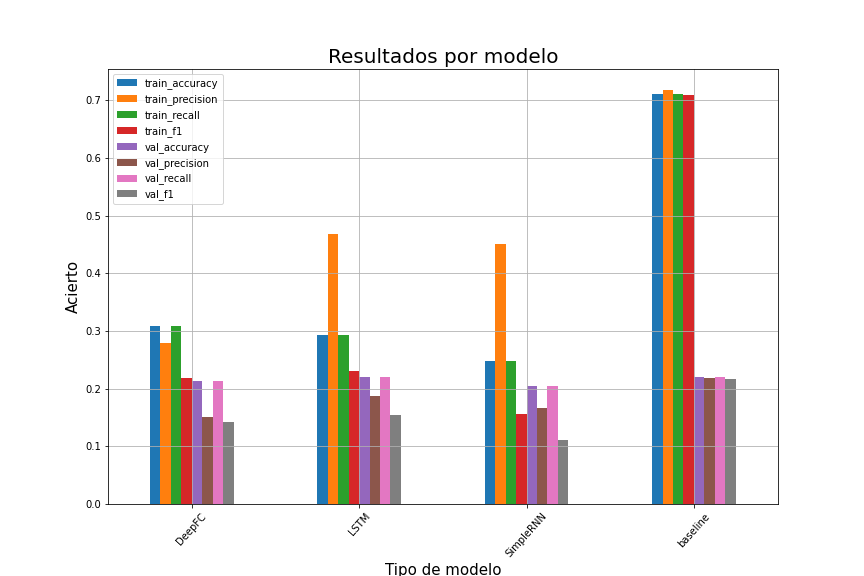
\includegraphics[width=0.9\textwidth]{results/friends/deepModels/sim_res_deep_model.png}
    \caption{Resultados por modelo}
    \label{fig:fri_deep_model}
\end{figure}

En el caso del tamaño del embedding implementado, los resultados son muy similares a los obtenidos para Los Simpson, en tanto a que a medida que se incrementa el embedding hay más posibilidad de sobre ajustar el modelo a los datos de entrenamiento.\\

\begin{figure}[H]
    \centering
    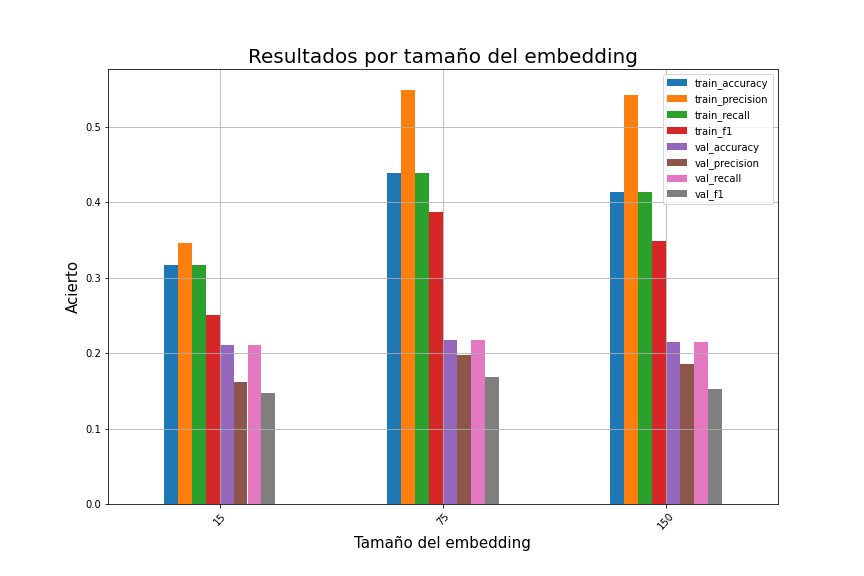
\includegraphics[width=0.9\textwidth]{results/friends/deepModels/sim_res_deep_em_size.png}
    \caption{Resultados por tamaño del embedding}
    \label{fig:fri_deep_em_size}
\end{figure}

Finalmente, en cuanto al tamaño de la secuencia, se observan resultados semejantes en validación con una pequeña diferencia en entrenamiento favoreciendo una secuencia de 15.\\

\begin{figure}[H]
    \centering
    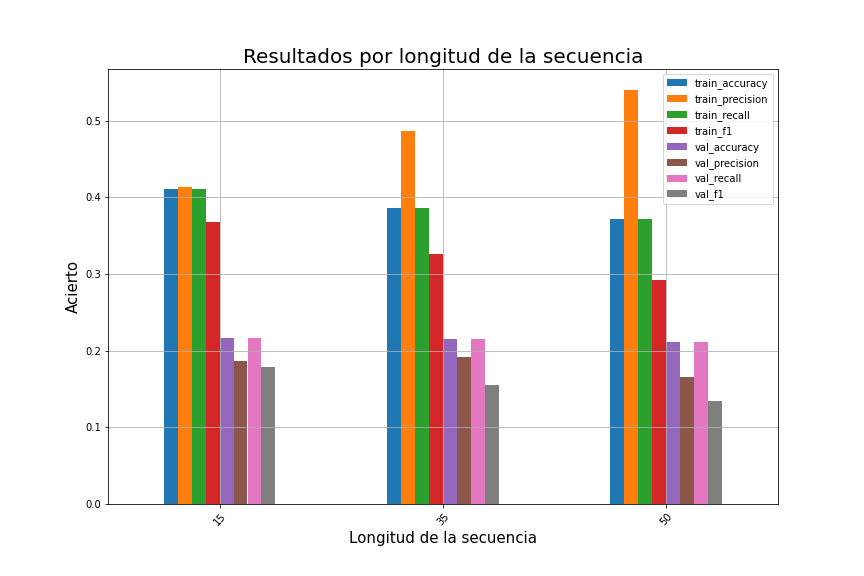
\includegraphics[width=0.9\textwidth]{results/friends/deepModels/sim_res_deep_seq_len.png}
    \caption{Resultados por tamaño de la secuencia}
    \label{fig:fri_deep_seq_len}
\end{figure}

Para análisis posteriores, se extrae el mejor modelo con base en el f1 score. Con este modelo se obtienen predicciones sobre datos de validación y de entrenamiento y se reentrena utilizando estos dos grupos de datos para predecir finalmente sobre los datos de test. Con base en todos estas predicciones se obtienen los siguientes resultados:

\begin{itemize}
    \item \textbf{Entrenamiento:}
    \input{results/friends/deepModels/Train.txt}

    \begin{figure}[H]
        \centering
        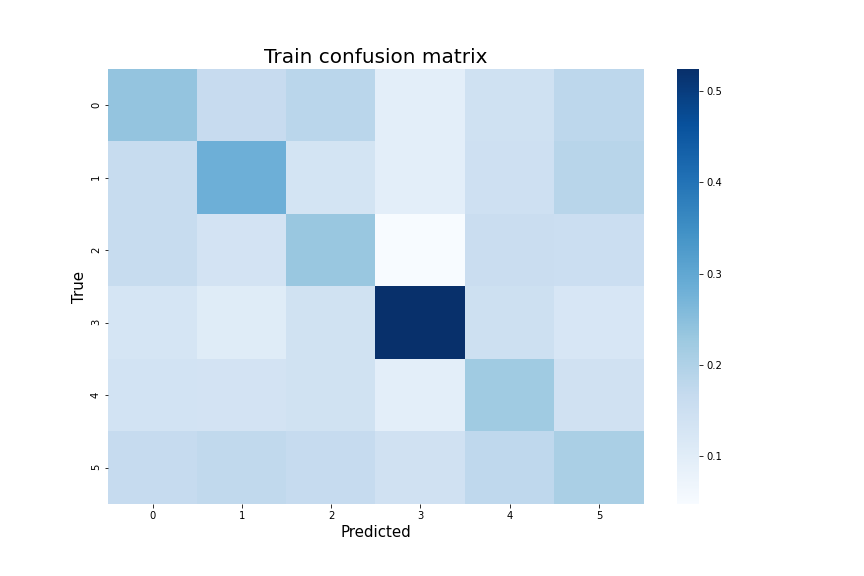
\includegraphics[width = 0.9\textwidth]{results/friends/deepModels/Train.png}
        \caption{Matriz de confusión para entrenamiento de friends}
        \label{fig:my_label}
    \end{figure}
    
    Es claro entonces que hay unas clases cuya precisión es muy alta mientras que su recall es bajo (Joey, Mónica) y por el contrario una clase cuyo recall es alto y su precisión es baja (Chandler). Esto quiere decir que el modelo casi identifica bastantes guiones de Chandler, pero podría decirse que lo asigna como por defecto, pues pocos de los que clasifica como suyos son realmente de su clase. En los restantes personajes sucede que el recall es bajo, mostrando que recupera pocos guiones de los que en realidad son de cada clase. En la matriz de confusión puede verse que la diagonal no resalta, pues hay muchos números de magnitud similar, indicando que el desempeño del modelo es muy aleatorio.

    \item \textbf{Validación:}
    \input{results/friends/deepModels/Validation.txt}

    \begin{figure}[H]
        \centering
        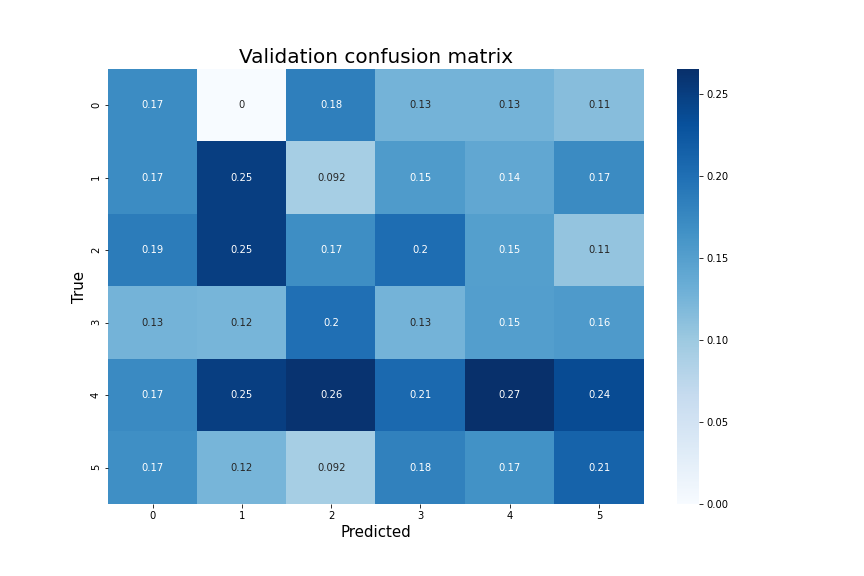
\includegraphics[width = 0.9\textwidth]{results/friends/deepModels/Validation.png}
        \caption{Matriz de confusión para validación de friends}
        \label{fig:my_label}
    \end{figure}
    
    Ahora bien, los resultados descritos previamente se repiten para el caso de validación como era de esperarse. Mostrando que las funciones que describen los datos de entrenamiento y validación son similares, dando lugar a una baja varianza. La matriz de confusión resulta muy mala en especial para la clase 4 donde clasifica sus diálogos como de otros con casi igual probabilidad.
    
    \item \textbf{Test:}
    \input{results/friends/deepModels/Test.txt}

    \begin{figure}[H]
        \centering
        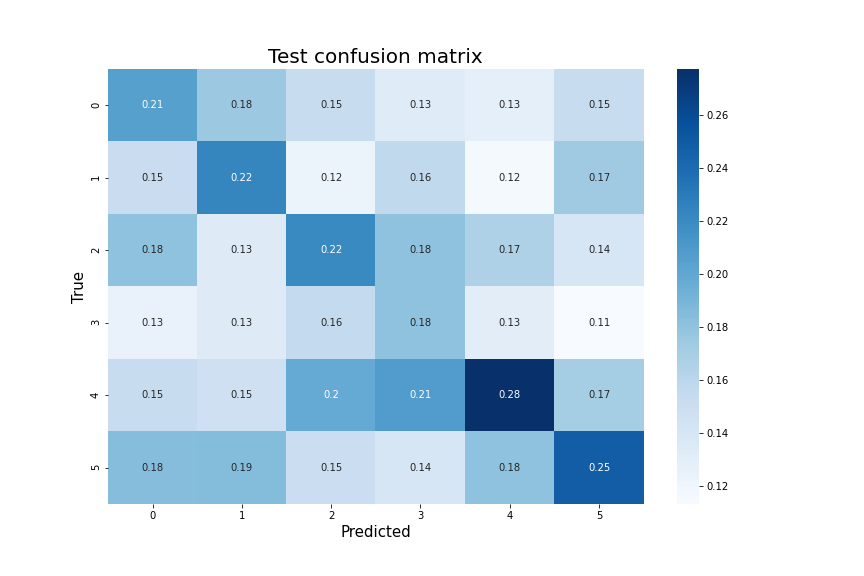
\includegraphics[width = 0.9\textwidth]{results/friends/deepModels/Test.png}
        \caption{Matriz de confusión para Test de friends}
        \label{fig:my_label}
    \end{figure}
    
    Para este caso es pertinente resaltar que, como se describió previamente, se utilizan los datos de entrenamiento y validación para entrenar nuevamente el modelo y se evalúa sobre los datos de test. Es evidente que el resultado de la clasificación es mejor que en las etapas previas, pues la diagonal de la matriz está más cargada.

\end{itemize}



\subsubsection{Modelos con embedding dentro de la red}
La tabla \ref{tab:em_friends_global} presenta los resultados de los tipos de modelos considerados para el problema de clasificación del conjunto de datos de \textit{Friends}. Los resultados de la tabla \ref{tab:em_friends_global} provienen de la evaluación del conjunto de prueba sobre el mejor modelo de cada uno de los tipos que fueron puestos a prueba. En términos generales se puede decir que los modelos logran captar suficiente información como para realizar una clasificación dado que su \textit{accuracy} es mayor del 16.33\% esperado en un clasificador completamente aleatorio. Por otra parte, se tienen los valores de \textit{precision} y \textit{recall} que se combinan en la puntuación F1. Para la \textit{precision} se puede notar que supera el 40\% para todos los tipos de modelos, lo cual indica que estos tienden a presentar un mayor número de falsos positivos. Sin embargo, el \textit{recall}, que en ningún caso supera el 10\%, indica que los modelos tienden fuertemente a presentar falsos negativos.

\begin{table}[H]
    \centering
    \csvreader[%
    tabular={|c|c|c|c|c|},
    table head=\hline \textbf{Modelo} & \textbf{Accuracy} & \textbf{Precision} & \textbf{Recall} & \textbf{F1} \\ \hline,
    late after line=\\ \hline,
    respect underscore = true
    ]%
    {data/results/friends_models.csv}%
    {model=\model, accuracy=\acc, precision=\prec, recall=\rec, F1=\fone}
    {\model & \acc & \prec & \rec & \fone}
    \caption{Métricas de evaluación sobre datos de prueba de \textit{Los Simpsons} para los mejores modelos de cada tipo.}
    \label{tab:em_friends_global}
\end{table}

\begin{table}[H]
    \centering
    \csvreader[%
    tabular={|c|c|c|c|},
    table head=\hline \textbf{Clase} & \textbf{Precision} & \textbf{Recall} & \textbf{F1} \\ \hline,
    late after line=\\ \hline,
    respect underscore = true
    ]%
    {data/results/friends_train.csv}%
    {class=\class, precision=\prec, recall=\rec, F1=\fone}
    {\class & \prec & \rec & \fone}
    \caption{Métricas de evaluación sobre datos de entrenamiento de \textit{Friends} discriminadas por clase.}
    \label{tab:em_friends_train}
\end{table}


\begin{table}[H]
    \centering
    \csvreader[%
    tabular={|c|c|c|c|},
    table head=\hline \textbf{Clase} & \textbf{Precision} & \textbf{Recall} & \textbf{F1} \\ \hline,
    late after line=\\ \hline,
    respect underscore = true
    ]%
    {data/results/friends_val.csv}%
    {class=\class, precision=\prec, recall=\rec, F1=\fone}
    {\class & \prec & \rec & \fone}
    \caption{Métricas de evaluación sobre datos de validación de \textit{Friends} discriminadas por clase.}
    \label{tab:em_friends_train}
\end{table}


\begin{table}[H]
    \centering
    \csvreader[%
    tabular={|c|c|c|c|},
    table head=\hline \textbf{Clase} & \textbf{Precision} & \textbf{Recall} & \textbf{F1} \\ \hline,
    late after line=\\ \hline,
    respect underscore = true
    ]%
    {data/results/friends_test.csv}%
    {class=\class, precision=\prec, recall=\rec, F1=\fone}
    {\class & \prec & \rec & \fone}
    \caption{Métricas de evaluación sobre datos de prueba de \textit{Friends} discriminadas por clase.}
    \label{tab:em_friends_train}
\end{table}


\subsubsection{Conclusiones}